\subsubsection{Quản lý mã nguồn}
Trong quá trình phát triển hệ thống tạo chatbot chăm sóc khách hàng, nhóm sử dụng Git - một hệ thống quản lý phiên bản phân tán phổ biến, nhằm đảm bảo việc kiểm soát và theo dõi quá trình thay đổi mã nguồn hiệu quả. Git cho phép các thành viên trong nhóm làm việc song song trên nhiều nhánh (branch), dễ dàng tích hợp mã (merge), theo dõi lịch sử thay đổi (commit history) và xử lý xung đột khi làm việc nhóm.

Để lưu trữ và quản lý mã nguồn từ xa, nhóm lựa chọn GitHub - một nền tảng lưu trữ mã nguồn trực tuyến dựa trên Git. GitHub hỗ trợ nhiều tính năng hữu ích cho phát triển cộng tác như pull request, issue tracking, CI/CD tích hợp, và khả năng quản lý phân quyền truy cập theo từng repository.

Để tổ chức cấu trúc mã nguồn một cách rõ ràng và dễ quản lý, nhóm đã tạo một GitHub Organization với tên là CoolChat. Trong đó, mã nguồn của hệ thống được chia thành ba repository riêng biệt tương ứng với từng thành phần chức năng:
\begin{itemize}
    \item CoolChat-FE: chứa mã nguồn frontend, được phát triển bằng React và Vite.
    \item CoolChat-BE: chứa mã nguồn backend, được xây dựng bằng Django REST Framework.
    \item CoolChat-AI: chứa mã nguồn liên quan đến xử lý AI và tích hợp chatbot, bao gồm mô hình xử lý ngôn ngữ tự nhiên.
\end{itemize}
\begin{figure}[H]
	\centering
	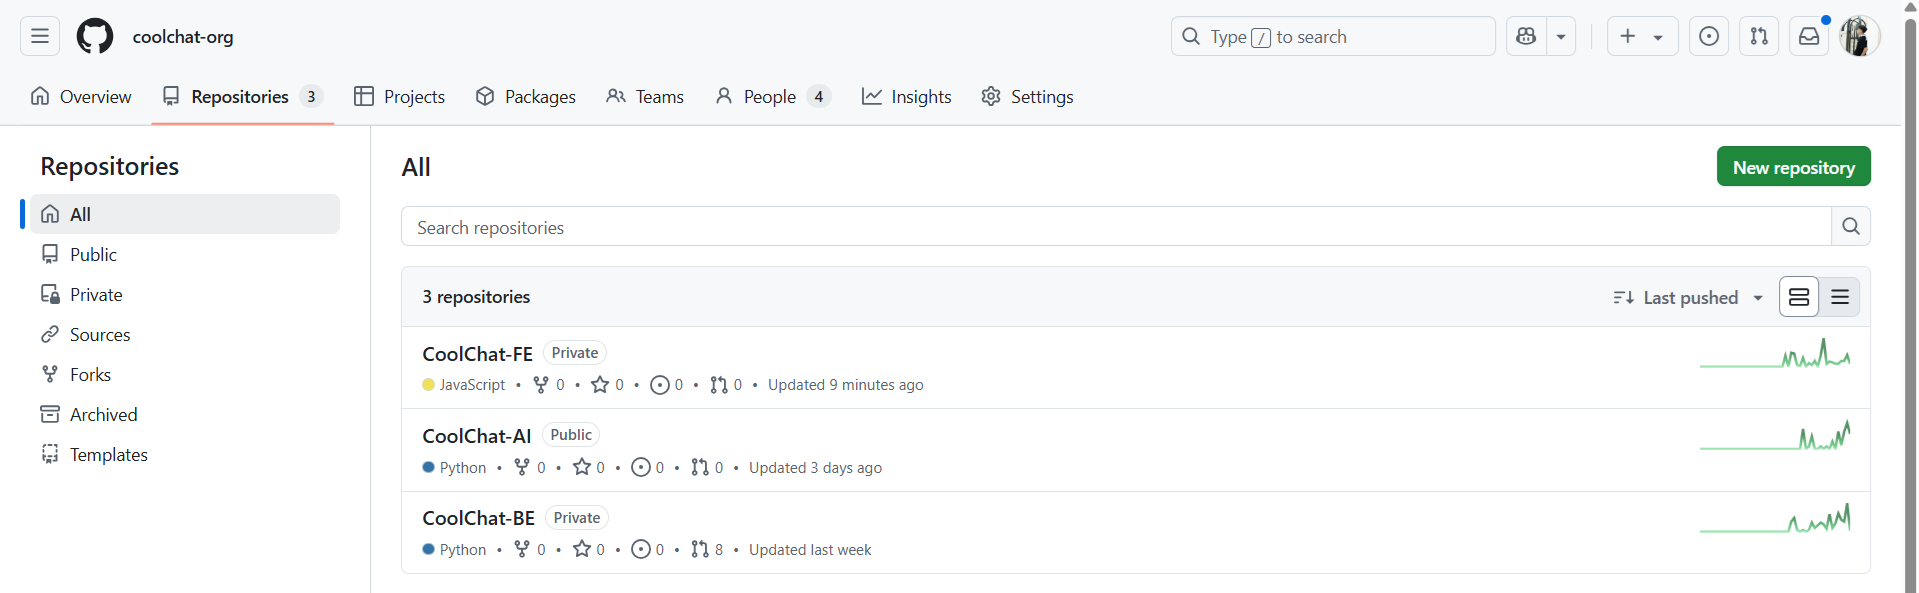
\includegraphics[width=1\textwidth]{Images/Implementation/git-org.png}
	\vspace{0.5cm}
	\caption{CoolChat Organization}
	\label{fig:enter-label}
\end{figure}

Cấu trúc tổ chức này giúp nhóm phân tách rõ ràng trách nhiệm phát triển, triển khai và bảo trì các thành phần hệ thống, đồng thời thuận tiện cho việc phân quyền truy cập, kiểm soát phiên bản và triển khai CI/CD độc lập cho từng phần.
\subsubsection{Cấu trúc mã nguồn}
\subsubsubsection{Frontend}
Cấu trúc mã nguồn Frontend như sau:
\begin{itemize}
    \item Các thư mục
    \begin{itemize}
        \item assets: Lưu trữ tài nguyên tĩnh như hình ảnh, icon, font,...
        \item components: Các thành phần UI tái sử dụng trong toàn bộ ứng dụng
        \item constants: Chứa các hằng số được dùng chung trong dự án, ví dụ: các giá trị cố định, config,...
        \item hooks: Các custom React hooks để tái sử dụng logic giữa các component
        \item i18n: Cấu hình và dữ liệu liên quan đến đa ngôn ngữ
        \item layouts: Các layout chung như layout cho trang chính, layout dashboard, layout xác thực,...
        \item pages: Các trang chính tương ứng với route trong ứng dụng
        \item services: Chứa các dịch vụ để giao tiếp với API với axios
        \item store: Quản lý trạng thái toàn cục với Redux
        \item utils: Các hàm tiện ích hỗ trợ cho nhiều phần trong dự án
    \end{itemize}
    \item Các file quan trọng
    \begin{itemize}
        \item App.jsx: File chính chứa cấu trúc cơ bản của ứng dụng (bao gồm router, provider,...)
        \item main.jsx: Điểm khởi chạy của ứng dụng React (ReactDOM.render) - nơi mount App vào DOM
        \item index.css: File CSS tổng cho toàn bộ app (chứa các style chung hoặc import từ Tailwind, ...)
        \item .env: File lưu trữ các biến môi trường
        \item .gitignore: Định nghĩa các file hoặc thư mục sẽ bị Git bỏ qua (không commit lên repository)
        \item eslint.config.js: Cấu hình ESLint để kiểm tra chuẩn code và format tự động
        \item index.html: File HTML gốc để React mount vào
        \item package.json: Khai báo các dependency, script, metadata của dự án
        \item package-lock.json: Ghi lại chính xác phiên bản các gói (dependencies) đã cài đặt để đảm bảo build đồng nhất
        \item postcss.config.js: Cấu hình PostCSS để xử lý CSS (kết hợp với TailwindCSS)
        \item README.md: Tài liệu hướng dẫn sử dụng, mô tả dự án
        \item tailwind.config.js: Cấu hình riêng cho TailwindCSS như theme màu sắc, breakpoint, plugin,...
        \item vercel.json: Cấu hình deploy trên nền tảng Vercel (hosting tự động)
        \item vite.config.js: Cấu hình Vite - quản lý alias, server, optimize,...
    \end{itemize}
\end{itemize}
\begin{figure}[H]
	\centering
	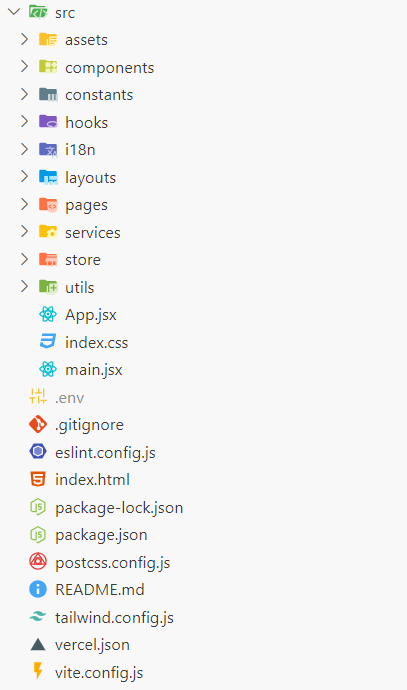
\includegraphics[width=0.4\textwidth]{Images/Implementation/fesource.png}
	\vspace{0.5cm}
	\caption{Cấu trúc mã nguồn Frontend}
	\label{fig:enter-label}
\end{figure}
\subsubsubsection{Backend}
\subsubsubsection{AI}
Cấu trúc mã nguồn của dịch vụ AI như sau:
\begin{itemize}
	\item Các thư mục
	\begin{itemize}
		\item .github: Chứa file .yml, đảm nhận việc CI/CD cho service trên Github Action.
		\item .venv: Chứa các gói thư viện cài đặt trong service.
		\item app: Là thư mục chính của service, chứa toàn bộ hiện thực mã nguồn.
		\item test: Chứa các bài kiểm thử về độ tin cậy của phản hồi từ chatbot.
	\end{itemize}

	\item Các module bên trong app:
	\begin{itemize}
		\item api: Là nơi định nghĩa các route và controller cho service. Các route xác định cách service phản hồi với các yêu cầu HTTP, trong khi controller xử lý logic để xử lý các yêu cầu đó.
		\item core: Là nơi khởi tạo các thiết lập, sự kết nối database. Đây là phần nền tảng để thiết lập môi trường cho service hoạt động.
		\item dtos: Là nơi tập trung của các data transfer object (DTO), dùng để giao tiếp giữa backend với service này. DTOs giúp chuẩn hóa định dạng dữ liệu trao đổi giữa các phần của hệ thống.
		\item middleware: Chứa các hàm middleware, có thể can thiệp vào yêu cầu và phản hồi để thực hiện xác thực trước khi yêu cầu đến controller.
		\item models: Chứa các model, đại diện cho cấu trúc dữ liệu và logic nghiệp vụ của ứng dụng. Các model thường tương ứng với các bảng trong cơ sở dữ liệu và bao gồm các phương thức để thao tác và xác thực dữ liệu.
		\item services: Chứa logic nghiệp vụ của service. Các service xử lý các hoạt động hoặc luồng công việc cụ thể, thường tương tác với các model để truy xuất hoặc cập nhật dữ liệu và thực hiện các tính toán hoặc xử lý cần thiết.
		\item utils: Chứa các hàm và lớp tiện ích. Đây là các đoạn mã có thể tái sử dụng cung cấp các chức năng chung, chẳng hạn như hàm trợ giúp cho việc thao tác chuỗi, định dạng ngày tháng, hoặc xử lý lỗi, có thể được sử dụng trong toàn bộ ứng dụng.
	\end{itemize}

	\item Các file quan trọng
	\begin{itemize}
		\item Dockerfile: Đây là file chỉ định quy cách đóng gói ứng dụng. Nó chứa các lệnh cần thiết để xây dựng một hình ảnh Docker cho ứng dụng, giúp đơn giản hóa việc triển khai và chạy ứng dụng trong một container.
		\item server.py: File khởi động server, đóng vai trò là điểm bắt đầu của ứng dụng.
		\item uv.lock: File sinh bởi trình quản lý gói 'uv', đảm bảo rằng các phiên bản của phụ thuộc được sử dụng là nhất quán giữa các môi trường khác nhau.
		\item pyproject.toml: File cấu hình cho dự án Python, thường được sử dụng bởi các công cụ như Poetry. File này chứa thông tin về phụ thuộc, cấu hình dự án, và metadata, giúp quản lý dự án khi không thể cài đặt uv.
		\item \_\_init\_\_.py: File này được sử dụng để biến một thư mục thành một gói Python, cho phép import các module từ thư mục đó. Nó có thể để trống hoặc chứa mã khởi tạo cho gói.
	\end{itemize}
\end{itemize}
\begin{figure}[H]
	\centering
	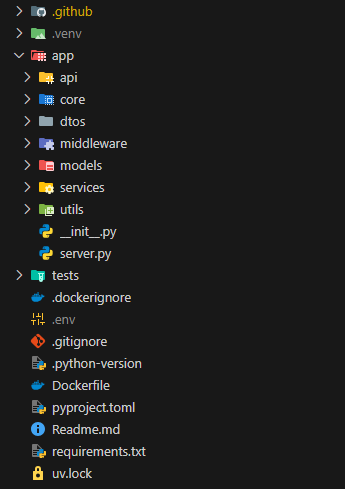
\includegraphics[width=0.4\textwidth]{Images/Implementation/aisource.png}
	\vspace{0.5cm}
	\caption{Cấu trúc mã nguồn AI Service}
	\label{fig:enter-label}
\end{figure}
